
\documentclass[12pt, addpoints]{exam}
\usepackage[utf8]{inputenc}
\usepackage[portuguese]{babel}
\usepackage{multicol}
\usepackage{graphicx}
\usepackage{amsmath}
\usepackage{xcolor}
\usepackage{tikz,pgfplots,tikz-3dplot,bm}
\usepackage{circuitikz}
\usepackage{tkz-base}
\usepackage{tkz-fct}
\usepackage{tkz-euclide}
\usepackage[a4paper, portrait, margin=2cm]{geometry}

\usetikzlibrary{arrows,3d,calc,automata,positioning,shadows,math,fit,shapes}
\usetikzlibrary{patterns,hobby,optics,calc}
\setlength{\columnsep}{1cm}
\renewcommand{\choiceshook}{\setlength{\leftmargin}{0pt}}

        \begin{document}

        \begin{minipage}[b]{0.75\linewidth}
            \begin{flushleft}
                {\bf \large Prova bimestral}
            \end{flushleft}
            \begin{flushleft}
                {\bf \large LQ2N (2B), 31 de outubro de 2022}
            \end{flushleft}
        \end{minipage}
        \begin{minipage}[b]{0.20\linewidth}
            \begin{flushright}
                {\bf \large Código: 0}
            \end{flushright}
        \end{minipage}
        \vspace{0.5cm} \hrule \vspace{0.5cm}
        \begin{minipage}{0.75\linewidth}
            Aluno:
        \end{minipage}
        \vspace{0.5cm} \hrule \vspace{0.5cm}

        \begin{questions}
\begin{multicols*}{2}
\question[20] A figura abaixo mostra a trajetória de uma partícula carregada $\vec{v}$ representa a velocidade atravessando um campo magnético $\vec{B}$. Determine a sua trajetória devido a ação da força magnética atuando sobre ela.

\begin{center}
\begin{minipage}[c]{0.50\linewidth}
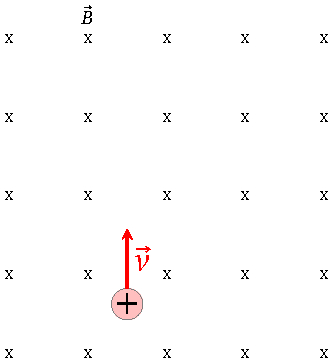
\includegraphics[width=\textwidth]{CEMAG001.jpg}
\end{minipage}
\end{center}
\begin{choices}
\choice Paralelo ao papel e da esquerda para a direita.\choice Paralelo ao papel e na vertical.\choice Paralelo ao papel e circular no sentido anti-horário.\choice Paralelo ao papel e da direita para a esquerda.\choice Paralelo ao papel e circular no sentido horário.\end{choices}
\question[20] Uma corrente elétrica de    6.79 A percorre um fio de cobre. Sabendo-se que a carga de um elétron é igual a $1,6\times 10^{-19}\;C$, qual é o número de elétrons que atravessa, por minuto, a seção reta desse fio?

\begin{oneparchoices}
\choice 9.8e+19;\choice 2.5e+21;\choice 2.5e+19;\choice 1.1e-18;\choice 4.2e+19;\choice 9.8e+19;\choice 6.5e-17;\choice 7.5e+19;\choice 5.8e+19;\choice 5.7e+19;\end{oneparchoices}
\question[20] Considere a figura abaixo onde as linhas trajeçadas representam superfícies equipotenciais Se colocarmos um elétron próximo a carga Q, quais trechos possíveis o elétron poderá se deslocar?
        
        \begin{center}
            \begin{minipage}[c]{0.5\linewidth}
                \begin{tikzpicture}[scale=0.5,transform shape, font=\Large]

                \tkzInit[xmin=-4,xmax=4,ymin=-4,ymax=4]
                \tkzClip[space=0.5]

                \tkzDefPoints{0/0/O,4/0/P}

                \foreach \x in {0.5,1.25,2.25,3,4}{
                    \tkzDrawCircle[R,dashed,color=gray!50](O,\x)
                }

                \foreach \y in {0,1,...,11}{
                    \tkzDefPointsBy[rotation= center O angle 30*\y](O,P){P1,P2}
                \draw[->, line width=1.0pt] (O) -- (P2);}

                \tkzDefPoints{3/0/a,4/0/b,0/4/c,0/3/d}

                \tkzDrawPoints[color=red,fill=red,size=0.3cm](a,b,c,d)

                \tkzDrawPoints(O)
                \tkzLabelPoints[above right,font=\Large](a,b,c,d)

                \node[circle, radius=0.25, ball color=gray!50] (n1) at (0,0) {Q};

                \end{tikzpicture}
            \end{minipage}
        \end{center}
        
        

\begin{choices}
\choice $c\rightarrow b$ ou $d\rightarrow a$\choice $b\rightarrow a\rightarrow d\rightarrow c$ ou $c\rightarrow d\rightarrow a\rightarrow b$\choice $a\rightarrow b$ ou $d\rightarrow c$\choice $b\rightarrow c$ ou $a\rightarrow d$\choice $b\rightarrow a$ ou $c\rightarrow d$\end{choices}
\question[20] Uma diferença de potencial de 120 V é aplicada a uma bomba d’água. Sabe-se que em funcionamento, o motor da bomba é percorrido por uma corrente de    2.02 A. Qual é a potência desenvolvida nesse motor?

\begin{oneparchoices}
\choice 1.1e+04W;\choice 1.4e+04W;\choice 2.6e+03W;\choice 2.6e+04W;\choice 242.521 W;\choice 3.2e+04W;\choice 3.5e+04W;\choice   0.017 W;\choice 490.139 W;\choice  59.376 W;\end{oneparchoices}
\question[20] Uma partícula de carga 6.81e-06 C é lançada em um campo magnético uniforme de    0.56 T , com uma velocidade de 2517.14 m/s. Calcule o valor da força magnética atuando na carga se o ângulo entre a velocidade e o campo magnético for   59.10 graus.

\begin{oneparchoices}
\choice   0.567 N;\choice   0.003 N;\choice   0.004 N;\choice   0.005 N;\choice 5.6e-04 N;\choice   0.003 N;\choice   0.005 N;\choice   0.002 N;\choice   0.017 N;\choice   0.008 N;\end{oneparchoices}
\end{multicols*}
\end{questions}
\newpage
        \begin{minipage}[b]{0.75\linewidth}
            \begin{flushleft}
                {\bf \large Prova bimestral}
            \end{flushleft}
            \begin{flushleft}
                {\bf \large LQ2N (2B), 31 de outubro de 2022}
            \end{flushleft}
        \end{minipage}
        \begin{minipage}[b]{0.20\linewidth}
            \begin{flushright}
                {\bf \large Código: 1}
            \end{flushright}
        \end{minipage}
        \vspace{0.5cm} \hrule \vspace{0.5cm}
        \begin{minipage}{0.75\linewidth}
            Aluno:
        \end{minipage}
        \vspace{0.5cm} \hrule \vspace{0.5cm}

        \begin{questions}
\begin{multicols*}{2}
\question[20] A figura abaixo mostra a trajetória de uma partícula carregada $\vec{v}$ representa a velocidade atravessando um campo magnético $\vec{B}$. Determine a sua trajetória devido a ação da força magnética atuando sobre ela.

\begin{center}
\begin{minipage}[c]{0.50\linewidth}
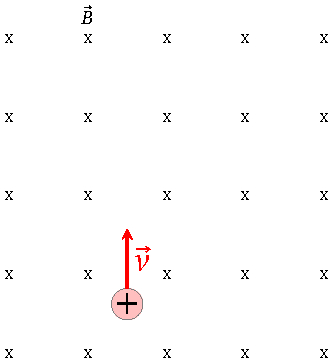
\includegraphics[width=\textwidth]{CEMAG001.jpg}
\end{minipage}
\end{center}
\begin{choices}
\choice Paralelo ao papel e da esquerda para a direita.\choice Paralelo ao papel e na vertical.\choice Paralelo ao papel e circular no sentido anti-horário.\choice Paralelo ao papel e da direita para a esquerda.\choice Paralelo ao papel e circular no sentido horário.\end{choices}
\question[20] Uma corrente elétrica de    6.79 A percorre um fio de cobre. Sabendo-se que a carga de um elétron é igual a $1,6\times 10^{-19}\;C$, qual é o número de elétrons que atravessa, por minuto, a seção reta desse fio?

\begin{oneparchoices}
\choice 9.8e+19;\choice 2.5e+21;\choice 2.5e+19;\choice 1.1e-18;\choice 4.2e+19;\choice 9.8e+19;\choice 6.5e-17;\choice 7.5e+19;\choice 5.8e+19;\choice 5.7e+19;\end{oneparchoices}
\question[20] Considere a figura abaixo onde as linhas trajeçadas representam superfícies equipotenciais Se colocarmos um elétron próximo a carga Q, quais trechos possíveis o elétron poderá se deslocar?
        
        \begin{center}
            \begin{minipage}[c]{0.5\linewidth}
                \begin{tikzpicture}[scale=0.5,transform shape, font=\Large]

                \tkzInit[xmin=-4,xmax=4,ymin=-4,ymax=4]
                \tkzClip[space=0.5]

                \tkzDefPoints{0/0/O,4/0/P}

                \foreach \x in {0.5,1.25,2.25,3,4}{
                    \tkzDrawCircle[R,dashed,color=gray!50](O,\x)
                }

                \foreach \y in {0,1,...,11}{
                    \tkzDefPointsBy[rotation= center O angle 30*\y](O,P){P1,P2}
                \draw[->, line width=1.0pt] (O) -- (P2);}

                \tkzDefPoints{3/0/a,4/0/b,0/4/c,0/3/d}

                \tkzDrawPoints[color=red,fill=red,size=0.3cm](a,b,c,d)

                \tkzDrawPoints(O)
                \tkzLabelPoints[above right,font=\Large](a,b,c,d)

                \node[circle, radius=0.25, ball color=gray!50] (n1) at (0,0) {Q};

                \end{tikzpicture}
            \end{minipage}
        \end{center}
        
        

\begin{choices}
\choice $c\rightarrow b$ ou $d\rightarrow a$\choice $b\rightarrow a\rightarrow d\rightarrow c$ ou $c\rightarrow d\rightarrow a\rightarrow b$\choice $a\rightarrow b$ ou $d\rightarrow c$\choice $b\rightarrow c$ ou $a\rightarrow d$\choice $b\rightarrow a$ ou $c\rightarrow d$\end{choices}
\question[20] Uma diferença de potencial de 120 V é aplicada a uma bomba d’água. Sabe-se que em funcionamento, o motor da bomba é percorrido por uma corrente de    2.02 A. Qual é a potência desenvolvida nesse motor?

\begin{oneparchoices}
\choice 1.1e+04W;\choice 1.4e+04W;\choice 2.6e+03W;\choice 2.6e+04W;\choice 242.521 W;\choice 3.2e+04W;\choice 3.5e+04W;\choice   0.017 W;\choice 490.139 W;\choice  59.376 W;\end{oneparchoices}
\question[20] Uma partícula de carga 6.81e-06 C é lançada em um campo magnético uniforme de    0.56 T , com uma velocidade de 2517.14 m/s. Calcule o valor da força magnética atuando na carga se o ângulo entre a velocidade e o campo magnético for   59.10 graus.

\begin{oneparchoices}
\choice   0.567 N;\choice   0.003 N;\choice   0.004 N;\choice   0.005 N;\choice 5.6e-04 N;\choice   0.003 N;\choice   0.005 N;\choice   0.002 N;\choice   0.017 N;\choice   0.008 N;\end{oneparchoices}
\end{multicols*}
\end{questions}
\newpage\end{document}